\documentclass{article}
\usepackage[margin=1in]{geometry} 
\usepackage{amsmath}
\usepackage[T1]{fontenc}          % change font encoding to T1
\usepackage{lmodern}  %better for visual on screen
\usepackage{graphicx}
\usepackage{float}
\usepackage{enumitem}
\usepackage{mathtools}
\usepackage{booktabs}
\usepackage{dirtree}

\makeatletter
\renewcommand*\env@matrix[1][\arraystretch]{%
	\edef\arraystretch{#1}%
	\hskip -\arraycolsep
	\let\@ifnextchar\new@ifnextchar
	\array{*\c@MaxMatrixCols c}}
\makeatother

% Used for adding Matlab Algorithms
\RequirePackage{listings}
\RequirePackage[framed,numbered]{matlab-prettifier}

\DeclarePairedDelimiter\abs{\lvert}{\rvert}%

\begin{document}
	\section{lsr.m}
	\lstinputlisting[
	label      = {alg:lsr},
	style      = Matlab-editor,
	basicstyle = \mlttfamily,
	firstline  = 1,
	lastline   = 49,
	firstnumber= 1
	]{../lsr.m}
	\subsection{Motivation/Concept}
	The function \textit{lsr.m} is a standalone matlab script that was written to perform least squares regression.  Matlab has built in functions \textit{lscov.m} for linear regression and \textit{nlinfit.m} for nonlinear regression. The MATLAB \textit{curve fitting toolbox} also has some optimization and regression fitting algorithms built in.  \textit{lsr.m} is intended to parallel the syntax of nlinfit, with the additional functionality to:
	\begin{itemize}
		\item perform total least squares
		\item perform linear least squares
		\item automatically detect linearity of the modelfun using numerical Hessian
		\item input analytical Jacobians
		\item perform $\chi^2$ Goodness of fit test to determine the significance of the computed reference variance $\sigma_0^2$
		\item disable covariance matrix scaling
		\item add an estimate of the beta coefficients as observation equations
	\end{itemize}
	
	\textbf{Linear and Nonlinear Least Squares} are used for systems of equations where the error is only in the dimension of the response variable and the optional stochastic model is only based on the uncertainty in the response variable.  These methods are not robust to outliers.
	
	\textbf{Total Least Squares} is used for linear and nonlinear systems of equations where the error is not solely in the dimension of the response variable.  When there is no stochastic model, this is also called orthogonal least squares, as the errors are perpendicular to the fit.  This method is useful when each of the measurements in the predictor variables have associated uncertainties or covariances.  This method is essentially iteratively re-weighting the system of equations by propagating uncertainty in each equation using GLOPOV to determine an estimated uncertainty in the response variable of each equation.  This method is not robust to outliers.
	
	\textbf{Robust Least Squares} is used for linear and nonlinear systems of equations where there are likely outliers.  A stochastic model may not be input.  A weight function iteratively re-weights the solution to reduce the influence of outliers.  Robust Least Squares does NOT provide a covariance and associated computed reference variance.  Matlab's nlinfit does, but I was uncomfortable duplicating that code because I didn't fully understand the assumptions being made.  
	
	\clearpage
	\subsection{Math}
	The observation equations are input as a function handle defined by the equation:
	\[
	y= F(\beta,x)
	\]
	Where:
	\begin{align*}
	y &= \text{Response Variables} \\
	F &= \text{model function (\textit{function y = modelfun(b,x)} in matlab)} \\
	\beta &= \text{Estimated Regression Coefficients} \\
	x &= \text{Predictor Variables}
	\end{align*}
	With Residuals(V) to account for uncertainty:
	\[
	V = F(\hat{\beta},x) - y
	\]
	The Least Squares Solution minimizes the sum of the square of the residuals:
	\[
	min\sum\limits_{i=1}^n v_i^2
	\]
	A stochastic model is introduced as a weight vector or a covariance matrix, where:
	\[
	\begin{cases}
	\text{No Weights or Covariance} & W = I \\
	\text{Weight Vector } (w) & W = diag(w)  \\
	\text{Covariance Matrix of Response Variables}(\Sigma_{yy}) & W = inv(\Sigma_{yy})
	\end{cases}
	\]
	\subsubsection*{Least Squares Assumptions Made}
	\begin{itemize}
		\item The system of equations is over-constrained
		\item Errors are normally distributed
		\item There are no outliers (Thought Robust attempts to handle them)
		\item Errors are not correlated with the magnitude of any of the predictor variables (what is this called?)
		\item others to add here? 
	\end{itemize}
	\subsubsection*{Automatic Partial Derivative Computation}
	The finite difference method is used to numerically compute the Jacobian Matrix of the model function with respect to the regression coefficients.  For Total Least Squares, the Jacobian of the model function with respect to the predictor variables is also computed.  The central finite difference is used, with the default $h$ equal to $eps^{\frac{1}{3}}$.  For increased accuracy, the user can input function handles for the $JacobianYB$ and $JacobianYX$, which eliminates the need for the numerical derivative calculations.
	
	\subsubsection*{Automatic Determination of Model Function Linearity}
	For linear functions, all of the elements of the Hessian should be equal to 0.  The Hessian is computed by performing the second partial numeric derivatives with respect to the regression coefficients for each observation, and comparing the values to 0. If all of the second derivatives are equal to 0, the model is linear.  As there could potentially be errors with this method, the user can also explicitly input the type of least squares to be performed.
	
	\subsubsection*{Optional inclusion of $\beta$ estimate as a set of observation equations}
	Sometimes, you can directly measure or estimate the predicted beta coefficients and their associated covariances.  For example, when attempting to triangulate a point using triginometry you may also have a low quality GPS coordinate and an associated covariance of that point.  This function allows you to pass in a covariance matrix for the beta parameter, which automatically adds it as an observation equation to further constrain the solution.
	
	In a simpler example, lets say we had 3 points with (x,y) coordinates and with a standard deviation of 5 in the y dimension.  We want to compute the slope and y intercept using $y=mx+b$.  The observation equations would look like:
	\begin{align*}
	&F_1:& y_1 + v_1 &= mx_1 + b \\
	&F_2:& y_2 + v_2 &= mx_2 + b \\
	&F_3:& y_3 + v_3 &= mx_3 + b
	\end{align*}
	But, somehow we also know that the slope should be $1\pm2$ and the y intercept should be $0.0 \pm 4$.  So we add two observation equations with the predicted values as extra response variables:
	\begin{align*}
	&F_4:& m_{est} + v_4 &= m \\
	&F_5:& b_{est} + v_5 &= b
	\end{align*}
	The A Matrix(Jacobian with respect to the regression coefficients) and the Covariance Matrix become:
	\[
	J_{y\beta} = 
	A = 
	\begin{bmatrix}[2.25]
	\dfrac{\partial F_1}{\partial m} & \dfrac{\partial F_1}{\partial b} \\
	\dfrac{\partial F_2}{\partial m} & \dfrac{\partial F_2}{\partial b} \\
	\dfrac{\partial F_3}{\partial m} & \dfrac{\partial F_3}{\partial b} \\
	\dfrac{\partial F_4}{\partial m} & \dfrac{\partial F_4}{\partial b} \\
	\dfrac{\partial F_5}{\partial m} & \dfrac{\partial F_5}{\partial b} \\
	\end{bmatrix}
	= 
	\begin{bmatrix}
	x_1 & 1 \\
	x_2 & 1 \\
	x_3 & 1 \\
	1 & 0 \\
	0 & 1 \\
	\end{bmatrix}
	\hspace{1cm}
	\Sigma_{yy} = 
	\begin{bmatrix}
	\sigma_{y_1}^2 & 0            & 0            & 0            & 0            \\
	0            & \sigma_{y_2}^2 & 0            & 0            & 0            \\
	0            & 0            & \sigma_{y_3}^2 & 0            & 0            \\
	0            & 0            & 0            & \sigma_{m_{est}}^2 & 0            \\
	0            & 0            & 0            & 0            & \sigma_{b_{est}}^2
	\end{bmatrix}
	= 
	\begin{bmatrix}
	5 & 0 & 0 & 0 & 0 \\
	0 & 5 & 0 & 0 & 0 \\
	0 & 0 & 5 & 0 & 0 \\
	0 & 0 & 0 & 2 & 0 \\
	0 & 0 & 0 & 0 & 4
	\end{bmatrix}
	\]
	
	\subsubsection*{$\chi^2$ Goodness of Fit Test (is $\sigma_0^2$ statistically equal to 1?)}
	A two tailed $\chi^2$ Goodness of Fit Test is used to determine if there is an issue with your least squares adjustment at an $\alpha$ significance level.  $\alpha$ values are normally low (eg. 0.01, 0.05).
	
	\begin{align*}
	\text{Null Hypothesis } H_0 &: S_0^2 = 1 \\
	\text{Alternative Hypothesis } H_a &: S_0^2 \neq 1 \\
	\text{Significance } &: \alpha
	\end{align*}
	Test Statistic:
	\[
	\chi^2 = \dfrac{vS_0^2}{\sigma^2} = \dfrac{dof\times S_0^2}{1} = dof\times S_0^2
	\]
	Rejection Region:
	\begin{align*}
	\chi^2 &< \chi_{(\alpha/2,dof)}^2 = \chi^2_{low} \\
	\chi^2 &> \chi_{(1-\alpha/2,dof)}^2 = \chi^2_{high} \\
	\end{align*}
	
	\clearpage
	\subsubsection*{Linear Least Squares}
	The equations to solve the estimated regression coefficient, $\hat{\beta}$, are given using:
	\begin{align*}
	A &= J_{y\beta} = \text{Partial Derivative of F with respect to }\beta \\
	WA\hat{\beta} &= Wy + WV\\
	\hat{\beta} &= (A^TWA)^{-1}A^TWy + WV\\
	\end{align*}
	Additional Linear Least Squares Parameters are computed using the following equations:
	\begin{align*}
	\text{Number of observations} &= m \\ 
	\text{Number of Regression Coefficients} &= n  \\
	\text{Degrees of freedom (\# of redundant observations)} &= dof = m-n \\
	\text{Weighted Residuals} &= WV = WA\hat{\beta} - Wy\\
	\text{Reference Variance} &= \sigma_0^2 = \dfrac{V^TWV}{dof} \\
	\text{Cofactor Matrix} &= Q_{yy} = inv(A^TWA) \\
	\text{Covariance Matrix of Unkowns} &= \Sigma_{yy} = \sigma_0^2 \times Q_{yy} \\
	\text{Covariance Matrix of Observations} &= \Sigma_{\hat{l}\hat{l}} = A \Sigma_{yy} A^T \\
	\text{Standard Deviation of Solved Unknowns} &= \sigma_{\hat{\beta}} = \sqrt{diag(\Sigma_{yy})} \\
	\text{Predicted y} &= \hat{y} = A\hat{\beta} = F(\hat{\beta},x)\\
	\text{R$^2$ (model skill)} &= \dfrac{var(\hat{y})}{var(y)} \\
	\text{RMSE } &= \sqrt{\dfrac{VV^T}{m}} \\
	\end{align*}
	
	\clearpage
	\subsubsection*{Nonlinear Loop Criteria}
	For Nonlinear Least Squares the solution is solved iteratively using an initial estimate for the $\beta$ coefficients.  The algorithm is coded to loop until either:
	\begin{enumerate}[label=\alph*)]
		\item the maximum iterations have been exceeded (default = 100)
		\item the computed reference variance $\sigma_0^2$ increases after an iteration, indicating a small change due to computer numerical precision.  *Note that this increase can also occur when the initial $\beta$ estimate is poor, of there is an error within the input data or model function.
	\end{enumerate}
	
	\subsubsection*{Nonlinear Least Squares}
	The loop equations to solve the estimated regression coefficient, $\hat{\beta}$, are given using:
	\begin{align*}
	i &= \text{while loop iteration number} \\
	K &= y - F(x,\hat{\beta_{i-1}}) \\
	WJ_{y\beta}\Delta\hat{\beta} &= WK + WV \\
	\Delta\hat{\beta} &= (J_{y\beta}^TWJ_{y\beta})^{-1}J_{y\beta}^TWK \\
	\hat{\beta}_i &= \hat{\beta}_{i-1} + \Delta\hat{\beta} \\
	V &= y - F(x,\hat{\beta_i}) \\
	\sigma_0^2 &= \dfrac{V^TWV}{dof}  
	\end{align*}
	Additional Nonlinear Least Squares Parameters are computed using the following equations:
	\begin{align*}
	\text{Number of observations} &= m \\ 
	\text{Number of Regression Coefficients} &= n  \\
	\text{Degrees of freedom (\# of redundant observations)} &= dof = m-n \\
	\text{Weighted Residuals} &= WV = WJ_{y\beta}\hat{\beta} - Wy\\
	\text{Reference Variance} &= \sigma_0^2 = \dfrac{V^TWV}{dof} \\
	\text{Cofactor Matrix} &= Q_{\beta\beta} = inv(J_{y\beta}^TWJ_{y\beta}) \\
	\text{Covariance Matrix of Unkowns} &= \Sigma_{\beta\beta} = \sigma_0^2 \times Q_{yy} \\
	\text{Standard Deviation of Solved Unknowns} &= \sigma_{\hat{\beta}} = \sqrt{diag(\Sigma_{yy})} \\
	\text{Predicted y} &= \hat{y} = F(\hat{\beta},x)\\
	\text{R$^2$ (model skill)} &= \text{Not valid for nonlinear least squares} \\
	\text{RMSE } &= \sqrt{\dfrac{VV^T}{m}} \\
	\end{align*}	
	\clearpage
	\subsubsection*{Total Least Squares Loop Criteria}
	The loop criteria for Total Least Squares is the same as for Nonlinear Least Squares.
	\subsubsection*{Total Least Squares}
	The loop equations to solve the estimated regression coefficients, $\hat{\beta}$, are given using:
	\begin{align*}
	V_{xx} &= \text{Residual of each observation} \\
	J_{yx} &= \text{Partial Derivative of F with respect to x} \\
	J_{yx}V_{xx} + J_{y\beta}\Delta\hat{\beta} &= K\\
	\Sigma_{xx} &= \text{Covariance of Predictor Variables} \\
	W_{eq} &= (J_{yx}\Sigma_{xx}J_{yx}^T)^{-1}\\
	V_{eq} &= \text{Equivalent Residuals} \\
	W_{eq}J_{y\beta}\Delta\hat{\beta} &= W_{eq}K + W_{eq}V_{eq} \\
	\Delta\hat{\beta} &= (J_{y\beta}^TW_{eq}J_{y\beta})^{-1}J_{y\beta}^TW_{eq}K \\
	\hat{\beta}_i &= \hat{\beta}_{i-1} + \Delta\hat{\beta} \\
	V_{eq} &= y - F(x,\hat{\beta_i}) \\
	\sigma_0^2 &= \dfrac{V_{eq}^TW_{eq}V_{eq}}{dof}  
	\end{align*}
	Additional Total Least Squares Parameters are computed using the following equations:
	\begin{align*}
	\text{Number of observations} &= m \\ 
	\text{Number of Regression Coefficients} &= n  \\
	\text{Degrees of freedom (\# of redundant observations)} &= dof = m-n \\
	\text{Residuals} &= V = \Sigma_{xx} J_{yx}^T W_{eq} V_{eq} \\
	\text{Reference Variance} &= \sigma_0^2 = \dfrac{V_{eq}^TW_{eq}V_{eq}}{dof} \\
	\text{Cofactor Matrix} &= Q_{\beta\beta} = inv(J_{y\beta}^TWJ_{y\beta}) \\
	\text{Covariance Matrix of Unkowns} &= \Sigma_{\beta\beta} = \sigma_0^2 \times Q_{yy} \\
	\text{Standard Deviation of Solved Unknowns} &= \sigma_{\hat{\beta}} = \sqrt{diag(\Sigma_{\beta\beta})} \\
	\text{Predicted y} &= \hat{y} = F(\hat{\beta},x)\\
	\text{R$^2$ (model skill)} &= \text{Not valid for nonlinear least squares} \\
	\text{RMSE } &= \sqrt{\dfrac{V_{eq}V_{eq}^T}{m}} \\
	\end{align*}
	
	\clearpage
	\subsubsection*{Robust Loop Criteria}
	The computation of the reference variance when performing Robust Least Squares is a bit challenging.  There is some literature on it, but it is currently not implemented in this function.  Therefore, searching for the first time the computed reference variance increases between iterations is no longer feasible.  As a replacement, the while loop exits on the following criteria:
	\begin{enumerate}[label=\alph*)]
		\item the maximum iterations have been exceeded (default = 100)
		\item the computed reference variance $\sigma_0^2$ changes by a value that is less than a threshold (default = 1e-8).
	\end{enumerate}
	\subsubsection*{Robust Least Squares}
	Robust Least Squares uses an iterative re-weighted method where the weight of each observation is determined by how large it's residual is.  The first iteration is solved with all weights equal to 1, then the residuals are normalized and converted to a weight using the robust weight function.  The normalization of the residuals and weight computations are given by the following equations:
	\begin{align*}
	\text{Hat Matrix: } H &= J_{y\beta} (J_{y\beta}^TJ_{y\beta})^{-1} J_{y\beta} \\
	\text{Leverages: }h &= diag(H) \\
	\text{Adjusted Residuals: }V_{adj} &= V*sqrt(h) \\
	\text{Ensure minimum residuals: }V_{adj} &= max(1e-6,V{adj}) \\
	\text{Estimated std (Median Absolute Residuals): }\hat{\sigma_{V_{adj}}} &= MAD(V_{adj})/0.6745 \\
	\text{Normalized Residuals: }V_{norm} &= V_{adj}/(RobustTune * {\sigma_{V_{adj}}}) \\
	\text{Weight Vector: }W &= RobustWgtFun(V_{norm}) \\
	\beta_i &= \text{Performed with either linear or nonlinear least squares}
	\end{align*}
	
	The statistics from Robust Least Squares solutions should be used with caution.  The iterative reweighting methodology effectively removes samples from influencing the dataset.  These "outliers" would significantly influence a computed RMSE.  Some would argue that Robust Least Squares isn't used as often because it is not "pure" least squares, in this sense, where it "sort of" includes outliers. 
	\clearpage
	\subsection{Input Variables}
	Below is a flowchart and table depicting how the type of least squares is determined and what input parameters apply to each type of least squares.
	
	\begin{figure}[H]
		\centering
		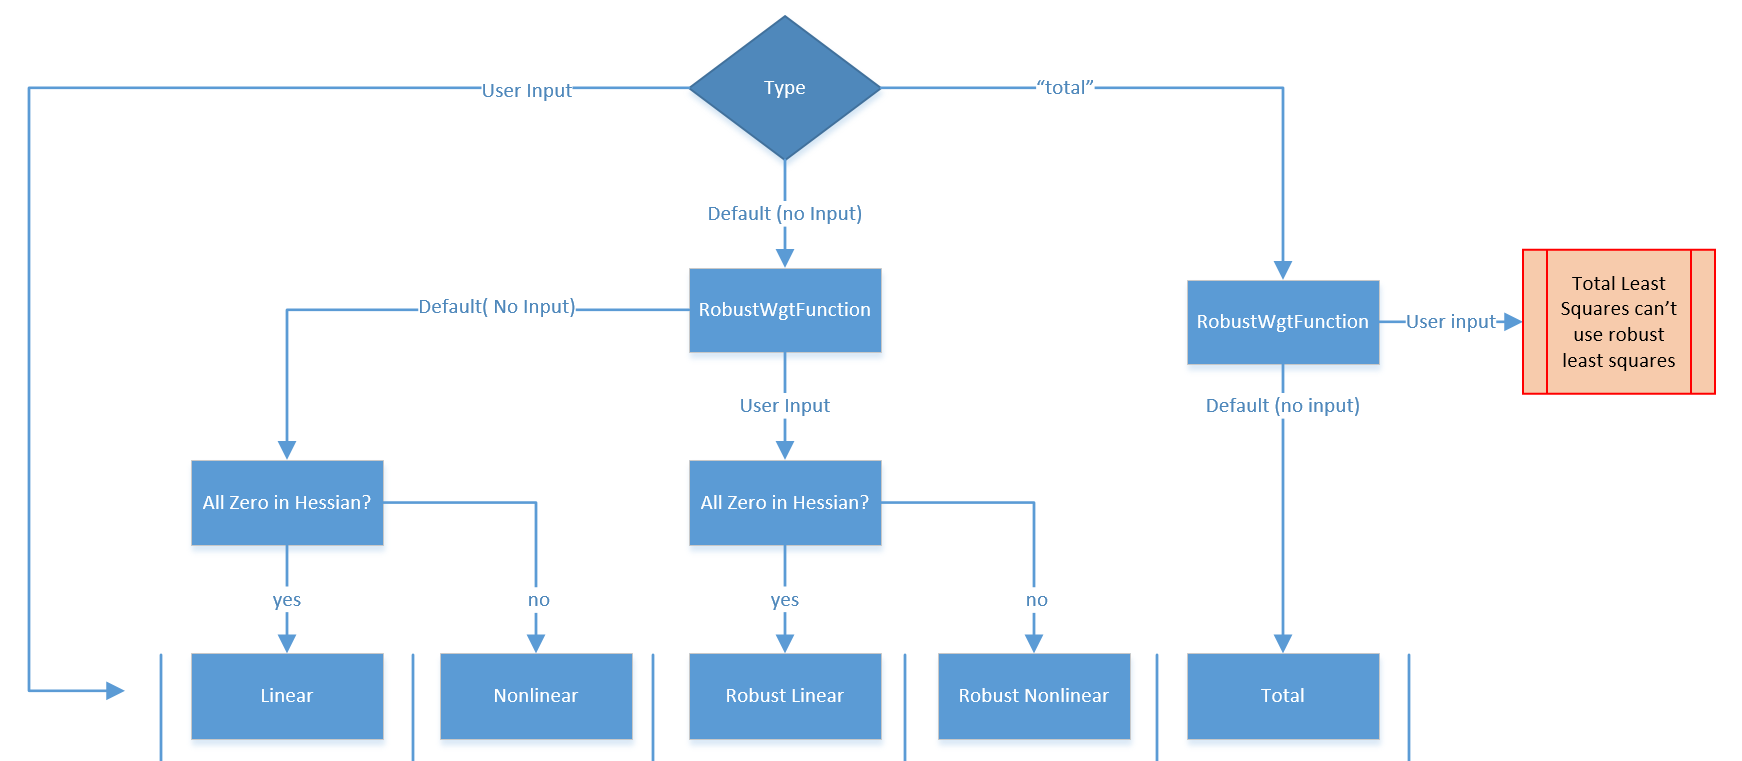
\includegraphics[width = \linewidth]{typeflow}
	\end{figure}
	\begin{figure}[H]
		\centering
		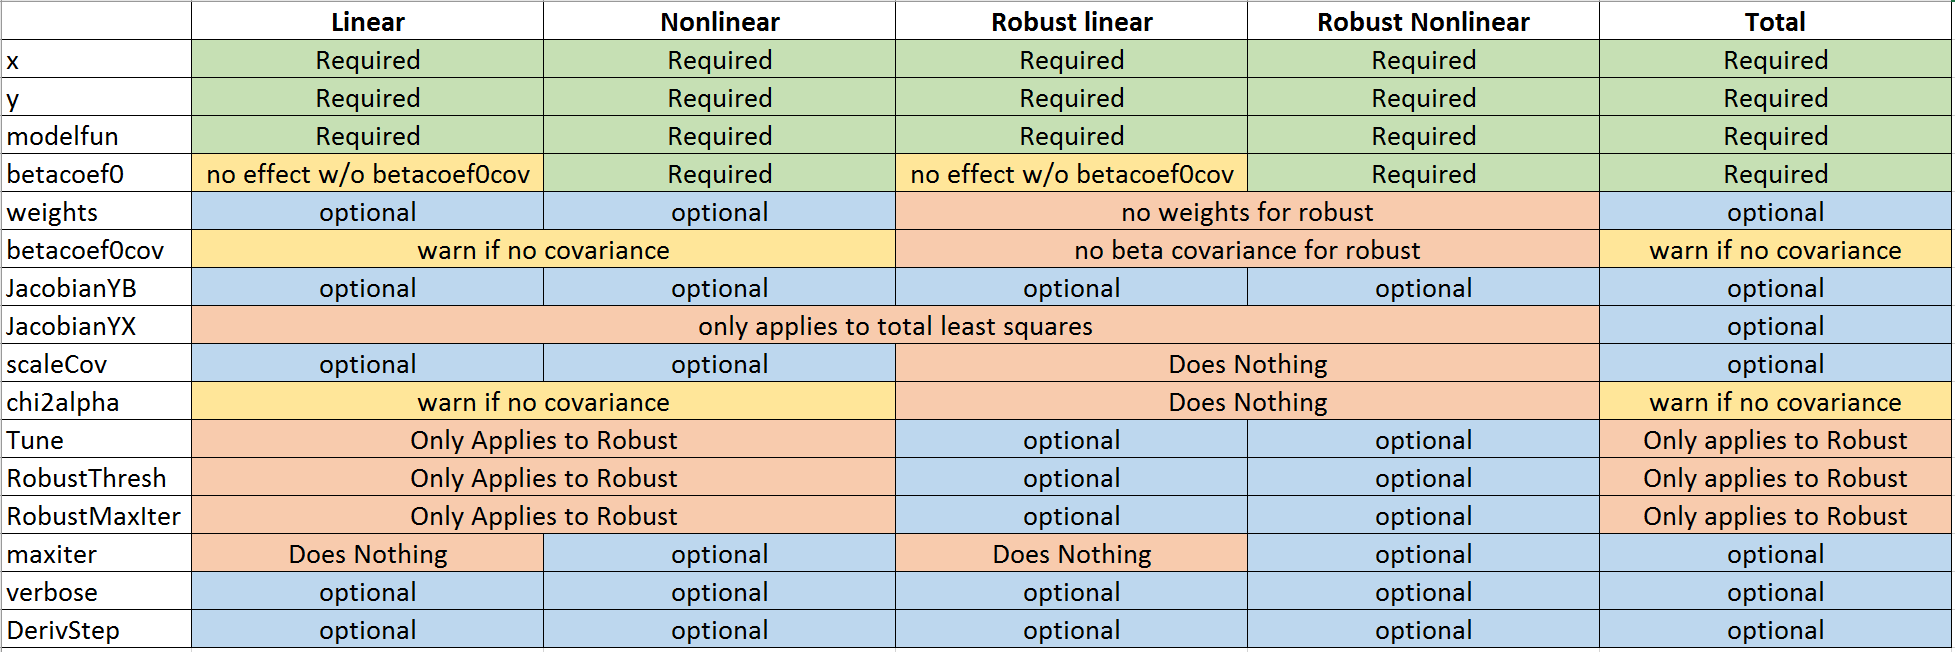
\includegraphics[width = \linewidth]{warningerrors}
	\end{figure}
	
	\subsubsection{x}
	Predictor variables
	
	The matrix \textit{x} is a matrix where each row is an observation, and the number of columns corresponds to the variables in the observation equation.
	\subsubsection{y}
	Response values
	
	The column vector \textit{y} of response values contains a row for each observation equation Size: [Nx1]
	\subsubsection{modelfun}
	Model function handle @modelfun(betacoef,x)
	
	The function handle \textit{modelfun} should take a regression coefficient input and x predictor variables matrix as inputs, and output a vector of response values.
	\subsubsection{betacoef0}
	Initial $\beta$ regression coefficient values
	
	\subsubsection{type}
	Type of Regression
	
	A string can be used to explicitly indicate the type of least squares to perform.  By default it is assumed that the model is either linear or nonlinear with the distinction computed using a numerical Hessian.
	\begin{table}[H]
		\begin{tabular}{l|l}
			\toprule
			Desired Type & Valid Input Strings \\
			\midrule
			linear & 'ols','wls','gls','lin','linear'\\
			nonlinear & 'nlin','nonlinear'\\
			robust linear & 'robustlinear','robust' (with modelfun Hessian = linear)\\
			robust nonlinear & 'robustnonlinear','robust' (with modelfun Hessian = nonlinear) \\
			total & 'total','tls'\\
			\bottomrule
		\end{tabular}
	\end{table}
	\subsubsection{weights}
	Vector (weights) or Covariance matrix
	
	A stochastic model is defined by either a vector of weights, or a covariance matrix.
	\[
	\begin{cases}
	\text{No Weights or Covariance (default)} & W = I \\
	\text{Weight Vector } (w) & W = diag(w)  \\
	\text{Covariance Matrix of Response Variables}(\Sigma_{yy}) & W = inv(\Sigma_{yy})
	\end{cases}
	\]
	\subsubsection{JacobianYB}
	Function @(b,x) for Jacobian with respect to the betacoef
	
	A function handle for the Jacobian of the modelfun with respect to the $\beta$ coefficients.  This function is normally not needed, as the numerical partial derivatives do a pretty good job.
	\subsubsection{JacobianYX}
	Function @(b,x) for Jacobian with respect to x
	
	A function handle for the Jacobian of the modelfun with respect to the $x$ predictor variables.  This function is normally not needed, as the numerical partial derivatives do a pretty good job.
	\subsubsection{noscale}
	Boolean (default:0) to scale covariance matrix
	
	By default, most least squares solutions will scale the covariance of the regression coefficients, $\Sigma_{\beta\beta}$, by the computed reference variance, $\sigma_0^2$.  If you have a high confidence that the initial reference variance is 1, then you can choose to not scale the covariance matrix with this flag.  The $\chi^2$ goodness of fit test will give insight into whether or not it is statistically valid to do this.
	
	\subsubsection{betaCoef0Cov}
	Covariance of beta0 coefficient values
	
	The covariance matrix of the initial beta coefficient values is used to add the estimates as observation equations, as described in the Math section above.
	\subsubsection{chi2alpha}
	Alpha values for significance
	
	The $\chi^2$ goodness of fit test uses an alpha value for the significance of the test.
	\clearpage
	\subsubsection{RobustWgtFun}
	Robust Weight Function
	
	The following functions are available as Robust Least Squares functions (Copied Directly From Matlab NLINFIT.M).  The user may also pass in a specific function handle instead.  
	\begin{table}[H]
		\begin{tabular}{llr}
			\toprule
			Weight Function & Equation                              & Default Tuning Constant \\
			\midrule
			'andrews'       & $w=I[\abs{r} < \pi] \times \sin(r)/r$ &                   1.339 \\
			'bisquare'      & $w=I[\abs{r}<1] \times (1-r^2)^2 $    &                   4.685 \\
			'cauchy'        & $w=\frac{1}{1+r^2} $                  &                   2.385 \\
			'fair'          & $w=\frac{1}{1+\abs{r}}$               &                   1.400 \\
			'huber'         & $w=\frac{1}{max(1,\abs{r})}$          &                   1.345 \\
			'logistic'      & $w=\frac{\tanh{r}}{r}$                &                   1.205 \\
			'talwar'        & $w=I[\abs{r}<1]         $             &                   2.795 \\
			'welsch'        & $w=e^{-r^2}$                          &                   2.985 \\
			\bottomrule
		\end{tabular}
	\end{table}
	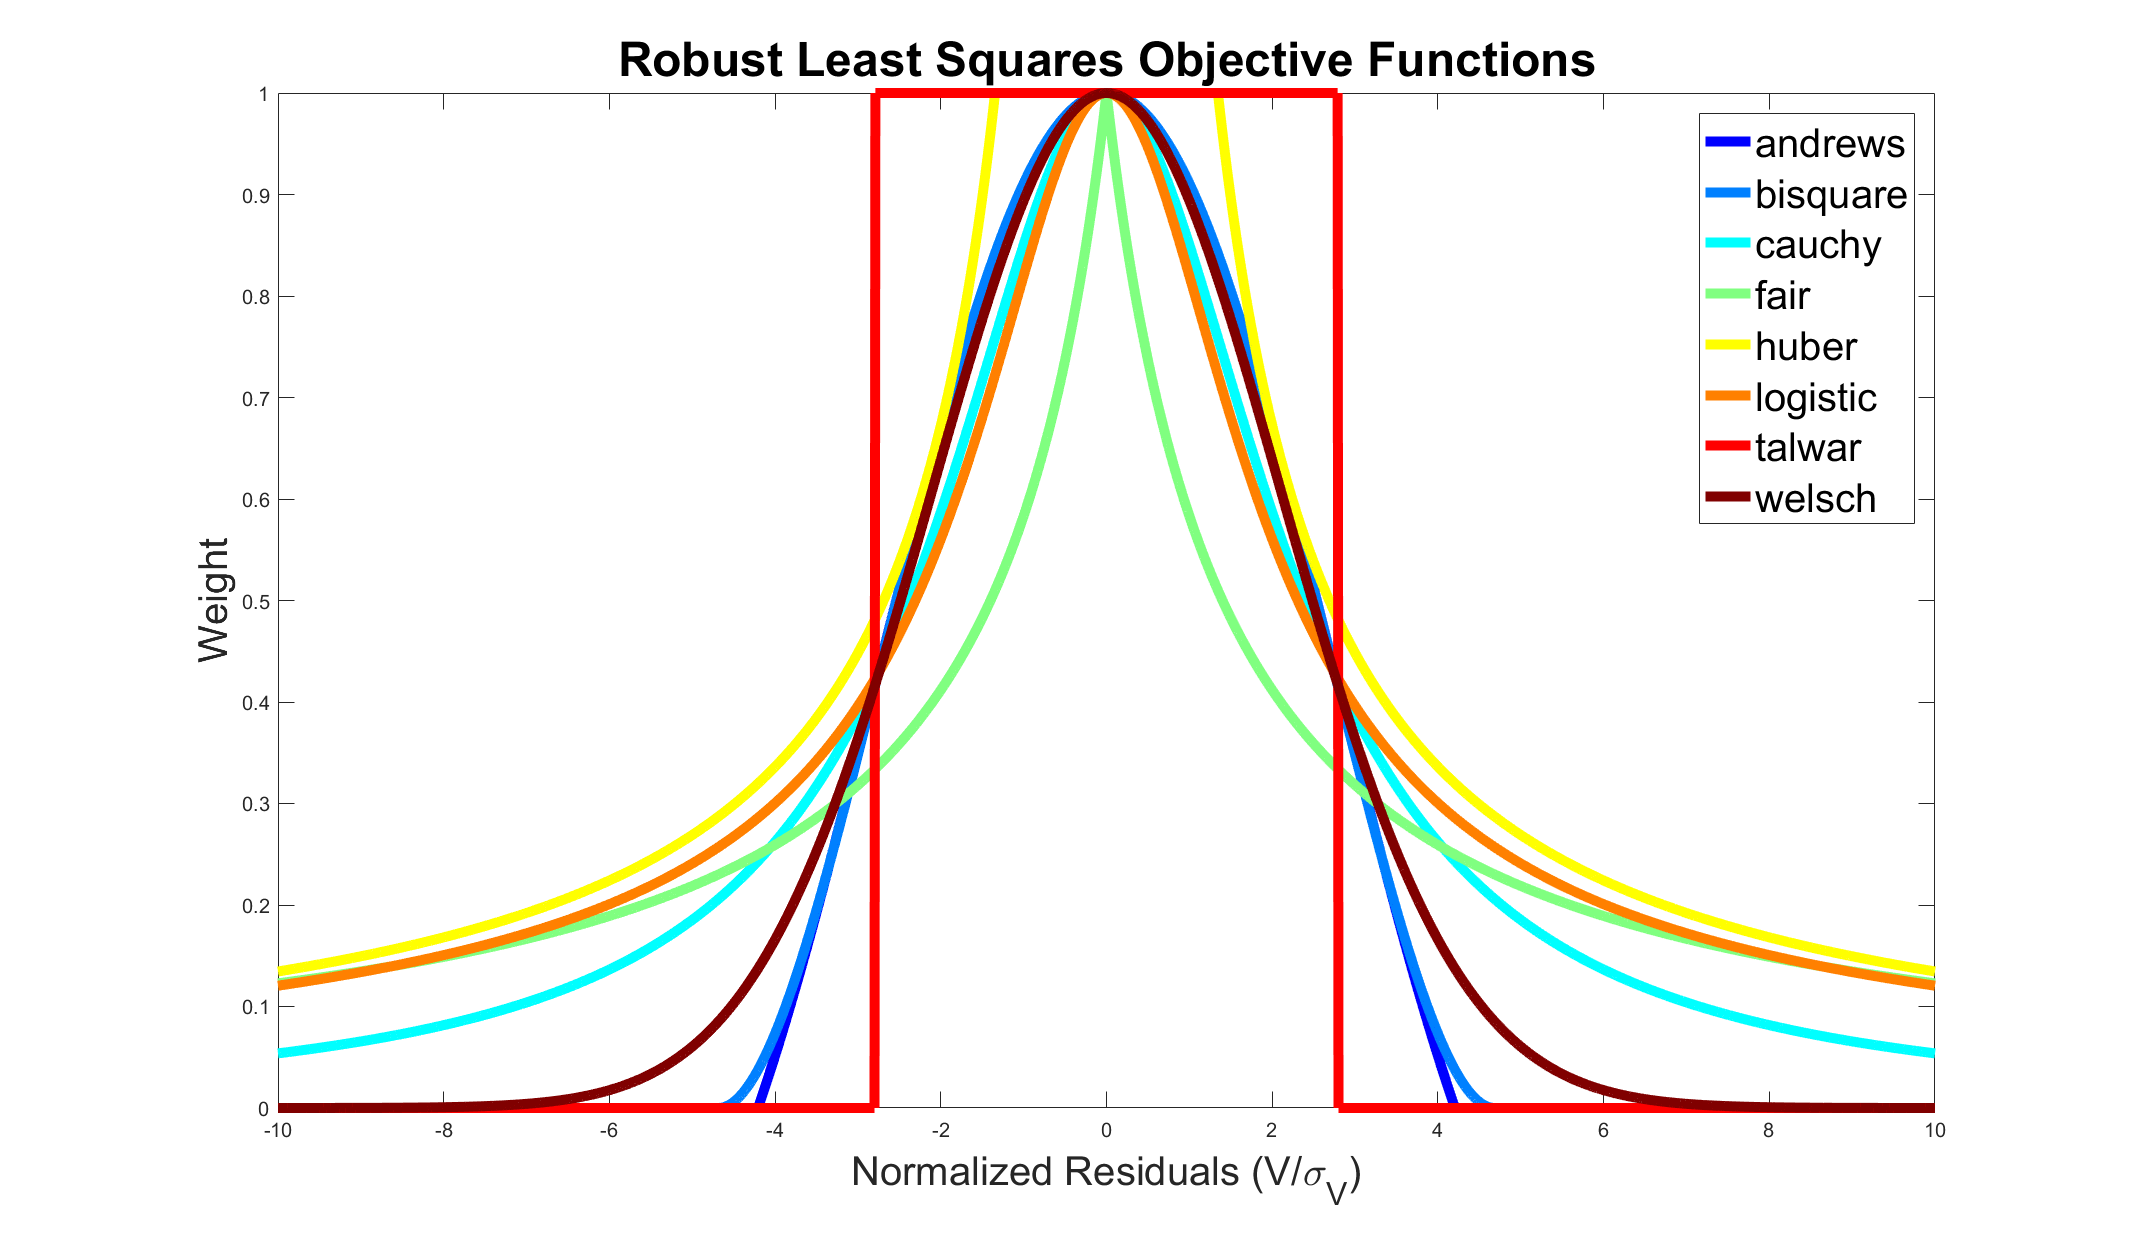
\includegraphics[width = \linewidth]{RobustFunctions}
	
	\subsubsection{Tune}
	Robust Weight Tuning Function
	
	The tune value adjusts the width of the robust function window.  A larger tune creates a broader window which will give more weight to higher residuals.
	\subsubsection{RobustThresh}
	Threshold for Robust Iterations
	
	The exit criteria for the robust loop is based on the there being a small change in the computed $\sigma_0^2$ between iterations that is smaller than the \textit{RobustThresh}.  The default value is 1e-8.
	\subsubsection{RobustMaxIter}
	Maximum iterations in Robust Least Squares (default = 100)
	
	\subsubsection{maxiter}
	Maximum iterations for Nonlinear (default = 100)
	
	\subsubsection{verbose}
	True/False print verbose output to screen
	
	\subsubsection{DerivStep}
	Difference for numerical Jacobian (default = $eps^{(1/3)}$)
	
	\subsubsection{enforceValidCovB}
	Logical flag to indicate if time should be spent attempting to make CovB a valid covariance matrix
	
	Sometimes the output covariance matrix can be either nonsymmetrical, or non positive semi definite, which indicates an invalid covariance matrix.  Basically rounding and other computer math errors results in a covariance matrix that is really really close to valid, but just a bit off.  A looping approach that chases its tail somewhat iteratively modifies the matrix to make it symmetrical, then positive semidefinite.  These steps sometimes affect the other, and it ends up looping until the math works.  It's not the best, but if you really need it, its there.  
	\subsection{Output Variables}
	\subsubsection{betacoef}
	Estimated regression coefficients
	
	\subsubsection{V}
	Weighted Residuals
	
	\subsubsection{J}
	Jacobian with respect to regression coefficients $\beta$
	
	\subsubsection{CovB}
	Estimated Variance Covariance Matrix of regression coefficients $\beta$
	
	\clearpage
	\subsubsection{modelinfo}
	Extra model data with the following structure:
	
	\dirtree{%
		.1 modelinfo.
		.2 type (type of regression).
		.2 nObservationEquations ($m$).
		.2 nBetaCoefficients ($n$).
		.2 dof (degrees of freedom).
		.2 betacoef ($\hat{\beta}$).
		.2 V (Weighted Residuals, $V_{eq}$ for total least squares).
		.2 R (Same as V for backwards compatability with nlinfit).
		.2 Vobs (Only for TLS, residual of each observation in x).
		.2 So2 ($\sigma_0^2$).
		.2 Q ($Q_{\hat{\beta}\hat{\beta}}$).
		.2 CovB ($\Sigma_{\hat{\beta}\hat{\beta}}$).
		.2 isCovBscaled (boolean for if CovB was scaled by So2 or not).
		.2 stdB ($\sigma_{\hat{\beta}}$ ).
		.2 r2 ($r^2$) .
		.2 RMSE (Root Mean Square Error).
		.2 Robust (only exists when robust regression is performed).
		.3 RobustWgtFun.
		.3 Tune.
		.3 RobustMaxIter.
		.3 RobustThresh.
		.3 niter.
		.2 niter (for nonlin or robust, number of iterations in loop).
		.2 chi2 (option $\chi^2$ tests when covariance matrix input).
		.3 alpha (significance level).
		.3 pass (boolean for if the $\chi^2$ goodness of fit test passed).
		.3 calculatedchi2 (computed $\chi^2$).
		.3 chi2low ($\chi^2_{low}$).
		.3 chi2high ($\chi^2_{high}$).
		.3 calculatedSo2 (computed $\sigma_0^2$).
		.3 So2low ($\chi^2_{low}/dof$).
		.3 So2high ($\chi^2_{high}/dof$).
			}
	
	\clearpage
	\subsection*{Example Usage (\textit{exampleLsr.m})}
	\subsubsection*{Fit Unweighted 2D Data with Different Models}
	This example demonstrates how to make an anonymous model function and call lsr with various models.
	\lstinputlisting[
	label      = {alg:lsr2},
	style      = Matlab-editor,
	basicstyle = \mlttfamily,
	firstline  = 2,
	lastline   = 22,
	firstnumber= 2
	]{../exampleLsr.m}
	
	
	\begin{figure}[H]
		\centering
		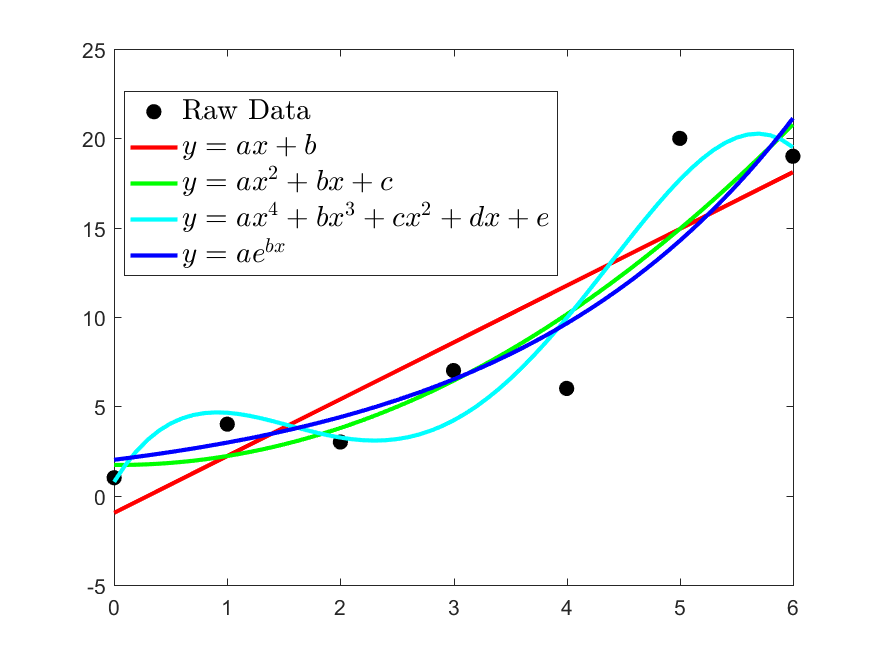
\includegraphics[height = 4in]{basicUsage}
	\end{figure}
	
	\clearpage
	\subsubsection*{Fit a Plane to 3D data}
	This example demonstrates fitting a plane to 3d points.  Notice how the predictor variables are input into matrix \textit{x} so that each row represents an observation.
	\lstinputlisting[
	label      = {alg:lsr2},
	style      = Matlab-editor,
	basicstyle = \mlttfamily,
	firstline  = 36,
	lastline   = 51,
	firstnumber= 36
	]{../exampleLsr.m}
	\begin{figure}[H]
		\centering
		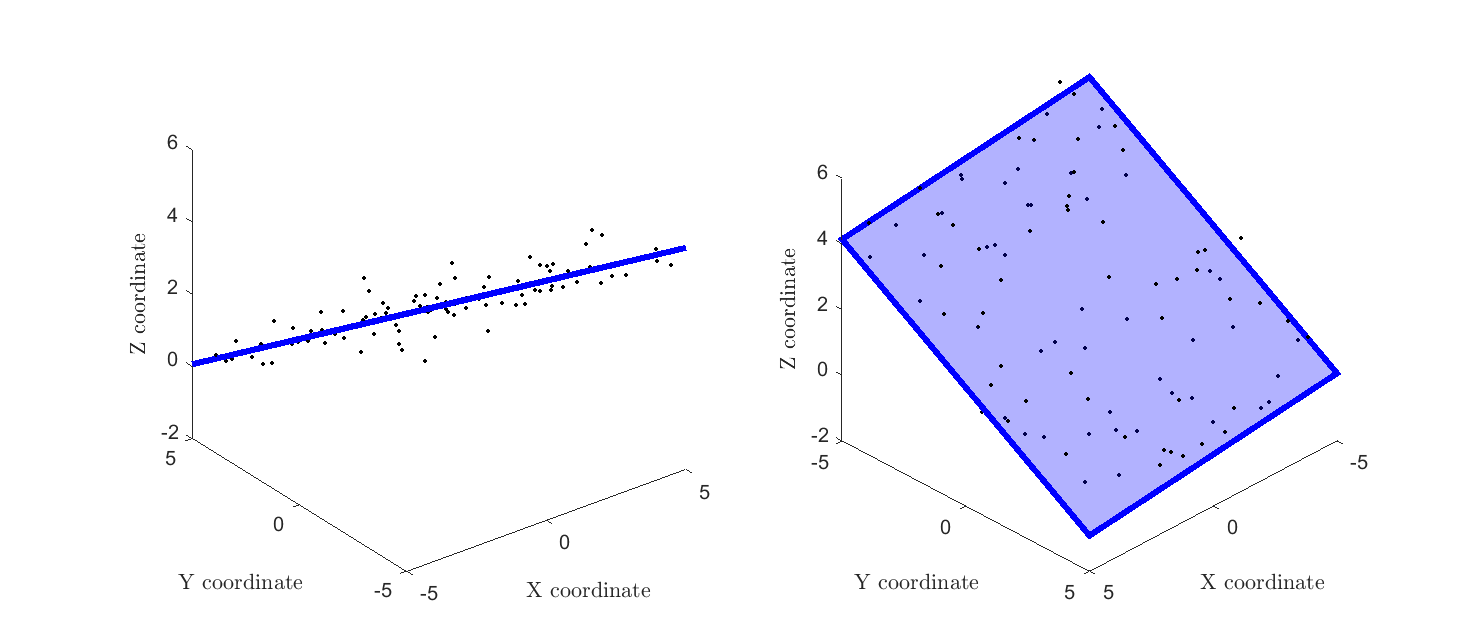
\includegraphics[width = \linewidth]{3dplane}
	\end{figure}
	\clearpage
	\subsubsection*{Sin Wave with known period}
	This example demonstrates how a sine wave can be fit as a linear or nonlinear model.  The results will be the same, but there is no need for an initial guess at the true beta in the linear case.
	\begin{align*}
	\text{NonLinear Function:  }y &= a\sin(\dfrac{2\pi}{T}x+\phi) \\
	\text{Linear Function:  }y &= a\sin(\dfrac{2\pi}{T}x) + b\cos(\dfrac{2\pi}{T}x)
	\end{align*}
	
	\lstinputlisting[
	label      = {alg:lsr2},
	style      = Matlab-editor,
	basicstyle = \mlttfamily,
	firstline  = 76,
	lastline   = 94,
	firstnumber= 76
	]{../exampleLsr.m}
	
	\begin{figure}[H]
		\centering
		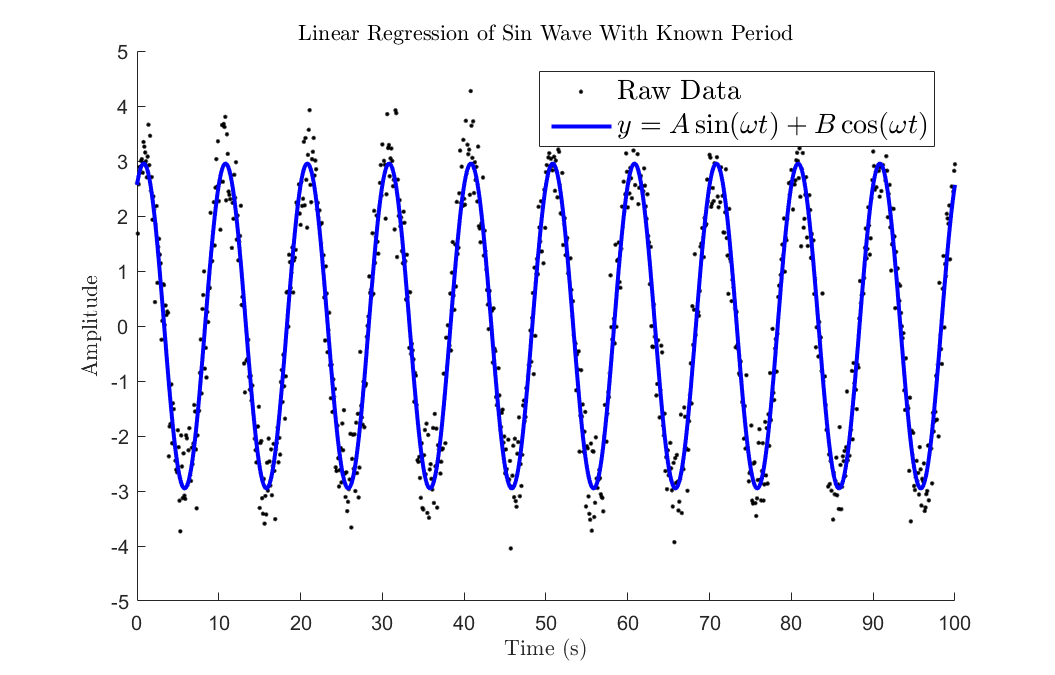
\includegraphics[width = \linewidth]{sin}
	\end{figure}
	
	\clearpage
	\subsubsection*{Different Ways to Weight Equations}
	This example demonstrate how to add a stochastic model to the least squares solution using either a weight vector or a covariance matrix.  The difference between the weighted solution and unweighted solution for a linear fit is shown in the figure.
	\lstinputlisting[
	label      = {alg:lsr2},
	style      = Matlab-editor,
	basicstyle = \mlttfamily,
	firstline  = 105,
	lastline   = 118,
	firstnumber= 105
	]{../exampleLsr.m}
	
	\begin{figure}[H]
		\centering
		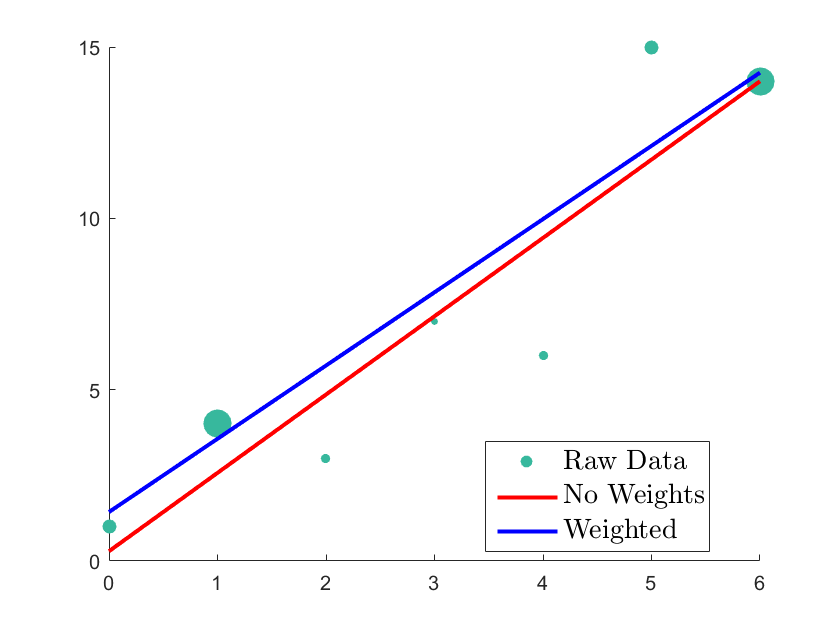
\includegraphics[width = \linewidth]{weights}
	\end{figure}
	
	\clearpage
	\subsubsection*{2D Conformal Coordinate Transformation}
	This example demonstrates how you can have a model function which handles multiple observation equations from the same set of data.  Notice that the function is also externally defined.
	
	\vspace{0.25cm}
	\noindent
	The 2D Conformal equations are:
	\begin{align*}
	X &= (S\cos(\theta))x - (S\sin(\theta))y + T_x \\
	Y &= (S\sin(\theta))x + (S\cos(\theta))y + T_y
	\end{align*}
	
	\noindent
	By substituting: 
	
	\begin{align*}
	a &= X\cos(\theta) \\
	b &= S\sin(\theta)
	\end{align*}
	Where:
	\begin{align*}
	\theta &= \tan^{-1}(\dfrac{b}{a}) \\
	S &= \dfrac{a}{\cos(\theta)}
	\end{align*}
	
	\noindent
	The observation equations become:
	
	\begin{align*}
	F: \hspace{1cm} X &= ax - by + T_x \\
	G: \hspace{1cm} Y &= bx + ay + T_y
	\end{align*}
	
	\noindent
	Note that every $(X,Y)\rightarrow(x,y)$ correspondence produces 2 observation equations.
	
	\lstinputlisting[
	label      = {alg:lsr2},
	style      = Matlab-editor,
	basicstyle = \mlttfamily,
	firstline  = 367,
	lastline   = 374,
	firstnumber= 367
	]{../exampleLsr.m}
	
	\lstinputlisting[
	label      = {alg:lsr2},
	style      = Matlab-editor,
	basicstyle = \mlttfamily,
	firstline  = 131,
	lastline   = 149,
	firstnumber= 131
	]{../exampleLsr.m}
	
	\clearpage
	\subsubsection*{Unweighted 3D Conformal Transformation}
	This example demonstrates a more complex 7-parameter 3D conformal transformation governed by the following equations:
	\[
	R = 
	\begin{bmatrix}
	r_{11} & r_{12} & r_{13} \\
	r_{21} & r_{22} & r_{23} \\
	r_{31} & r_{32} & r_{33} \\
	\end{bmatrix}
	=
	\begin{bmatrix}[1.5]
	\cos(\kappa)\cos(\phi) &
	\cos(\phi)\sin(\kappa) &
	-\sin(\phi) \\
	\cos(\kappa)\sin(\omega)\sin(\phi) - \cos(\omega)\sin(\kappa) &
	\cos(\kappa)\cos(\omega) + \sin(\kappa)\sin(\omega)\sin(\phi) &
	\cos(\phi)\sin(\omega) \\
	\sin(\kappa)\sin(\omega) + \cos(\kappa)\cos(\omega)\sin(\phi) &
	\cos(\omega)\sin(\kappa)\sin(\phi) - \cos(\kappa)\sin(\omega) &
	\cos(\omega)\cos(\phi) \\
	\end{bmatrix}
	\]
	\[
	\begin{bmatrix}
	X \\ Y \\ Z 
	\end{bmatrix}
	= 
	S\times
	R\times
	\begin{bmatrix}
	x \\ y \\ z
	\end{bmatrix}
	+ 
	\begin{bmatrix}
	T_x \\ T_y \\ T_z
	\end{bmatrix}
	\]
	
	Notice that a helper function is used to combine the X,Y,Z output from conformal 3D into a vector.  This satisfies the requirement that the response variables are in a column vector for input to \textit{lsr}.
	
	\lstinputlisting[
	label      = {alg:lsr2},
	style      = Matlab-editor,
	basicstyle = \mlttfamily,
	firstline  = 375,
	lastline   = 395,
	firstnumber= 375
	]{../exampleLsr.m}
	\clearpage
	Notice that using anonymous functions, it is very easy to choose which beta parameters to solve for.  In this example, the scale was set to 1, and the other 6 parameters were set as the regression coefficients.  
	\lstinputlisting[
	label      = {alg:lsr2},
	style      = Matlab-editor,
	basicstyle = \mlttfamily,
	firstline  = 151,
	lastline   = 173,
	firstnumber= 151
	]{../exampleLsr.m}
	
	\clearpage
	\subsubsection*{Linear Line with Total Least Squares}
	This example shows how to use total least squares.  The plot depicts how weighting a regression with total least squares is different than an unweighted solution, which should be fairly intuitive.  This is a simple example, however, and total least squares has advantages that are beyond the scope of this example.
	\lstinputlisting[
	label      = {alg:lsr2},
	style      = Matlab-editor,
	basicstyle = \mlttfamily,
	firstline  = 175,
	lastline   = 192,
	firstnumber= 175
	]{../exampleLsr.m}
	
	\begin{figure}[H]
		\centering
		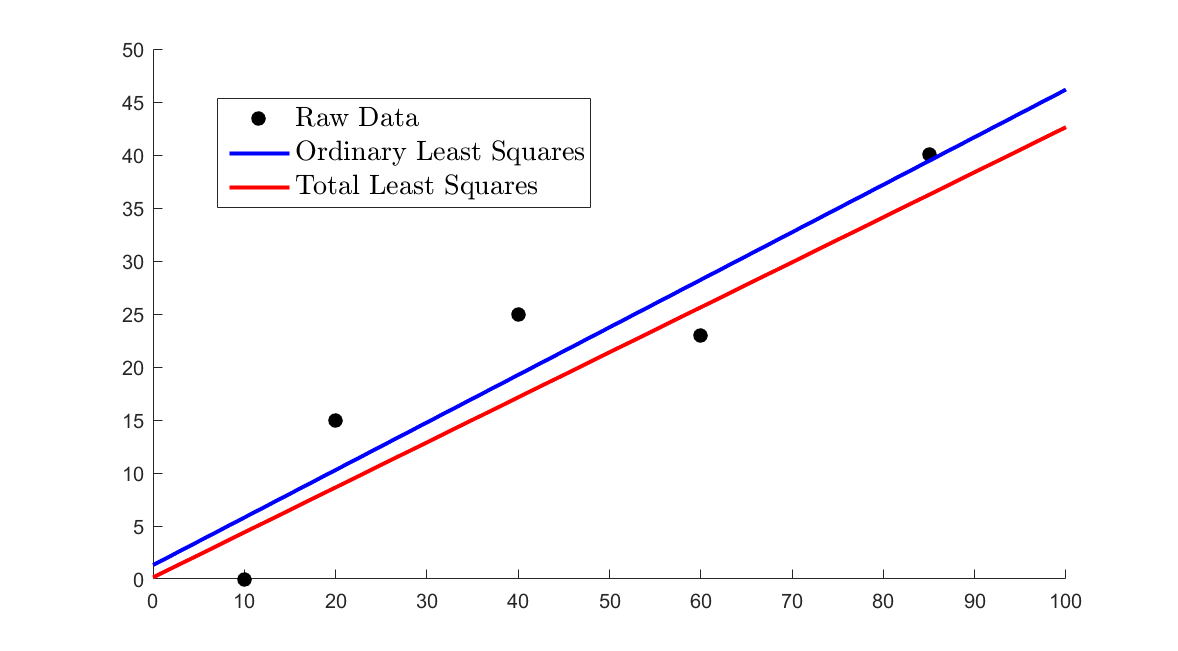
\includegraphics[width = \linewidth]{tls}
	\end{figure}
	
	\clearpage
	\subsubsection*{Robust Least Squares for Line with outliers}
	This example demonstrates how robust least squares is robust to outliers.
	
	\lstinputlisting[
	label      = {alg:lsr2},
	style      = Matlab-editor,
	basicstyle = \mlttfamily,
	firstline  = 204,
	lastline   = 214,
	firstnumber= 204
	]{../exampleLsr.m}
	
	\begin{figure}[H]
		\centering
		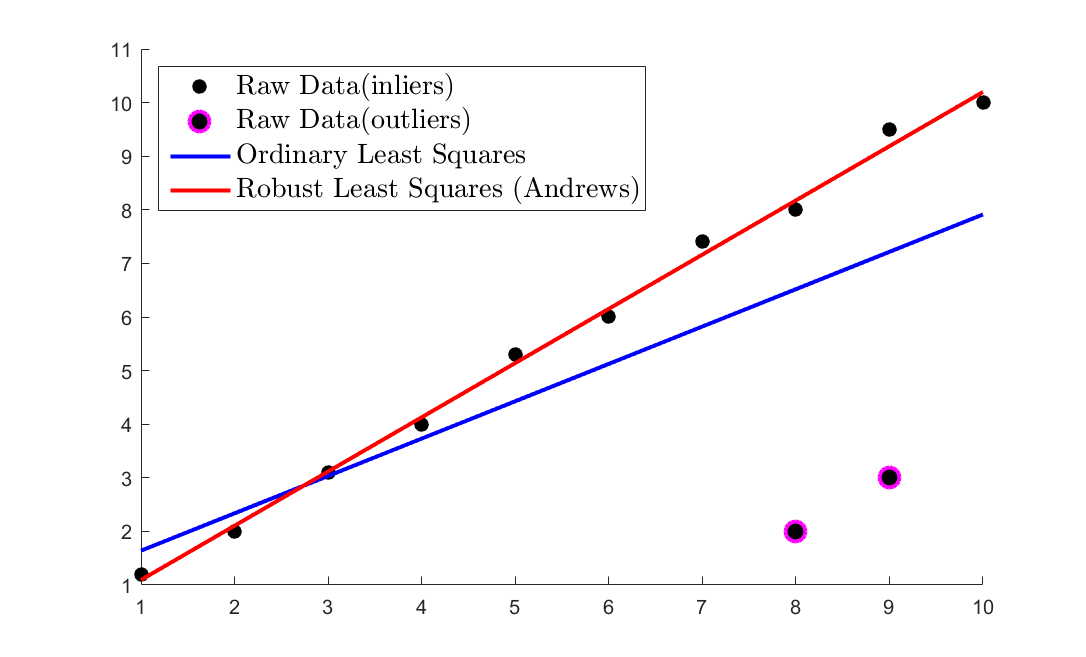
\includegraphics[width = \linewidth]{robust}
	\end{figure}
	
	\clearpage
	
	\subsubsection*{$\chi^2$ Goodness of Fit Test for linear line, Don't Scale Covariance}
	This example demonstrates how the $\chi^2$ Goodness of Fit Test can be used to see if it is valid to not scale the covariance matrix.  In this example, it is valid to not scale the covariance matrix.  The effect of poor estimation of input uncertainty and the effect of not scaling the covariance matrix are shown in the table shown. 
	\lstinputlisting[
	label      = {alg:lsr2},
	style      = Matlab-editor,
	basicstyle = \mlttfamily,
	firstline  = 226,
	lastline   = 245,
	firstnumber= 226
	]{../exampleLsr.m}
	
	\begin{figure}[H]
		\centering
		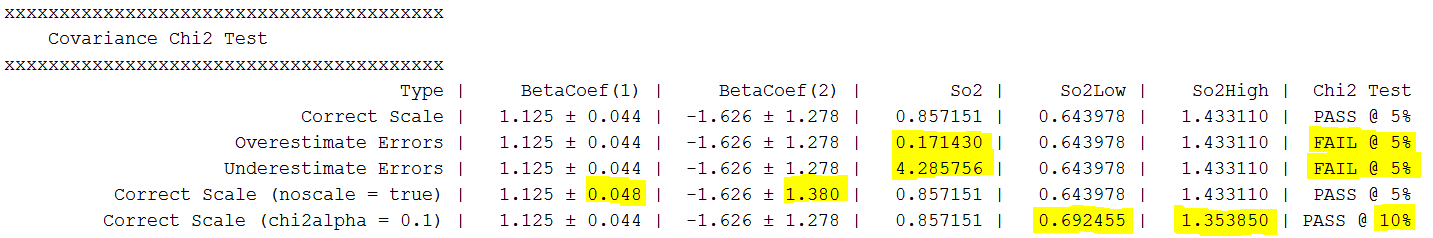
\includegraphics[width = \linewidth]{chi2}
	\end{figure}
	
	\clearpage
	\subsubsection*{Analytical Jacobians}
	This example demonstrates an example case when analytical Jacobian functions are input. Notice that because this is performing TLS, the t and z values must both be on the same side of the equation, and the resultant y response variables are all equal to 0.  The solution from numerical Jacobians and analytical Jacobians are almost exactly the same in this instance (within e-10), though the processing time for the analytical Jacobians was about twice as fast.  This speed increase will likely vary depending on the model function.    
	\lstinputlisting[
	label      = {alg:lsr2},
	style      = Matlab-editor,
	basicstyle = \mlttfamily,
	firstline  = 274,
	lastline   = 299,
	firstnumber= 274
	]{../exampleLsr.m}
	
	\clearpage
	\subsubsection{Use Regression Coefficient Estimate as Observation Equations}
	This example demonstrates how you can use the estimate of the regression coefficients as observation equations to influence the regression model.  Notice how the blue line, with the estimated regression coefficients used as observation equations, is closer to the green line, which is the line generated using the estimated regression coefficients.
	\lstinputlisting[
	label      = {alg:lsr2},
	style      = Matlab-editor,
	basicstyle = \mlttfamily,
	firstline  = 301,
	lastline   = 311,
	firstnumber= 301
	]{../exampleLsr.m}
	
	\begin{figure}[H]
		\centering
		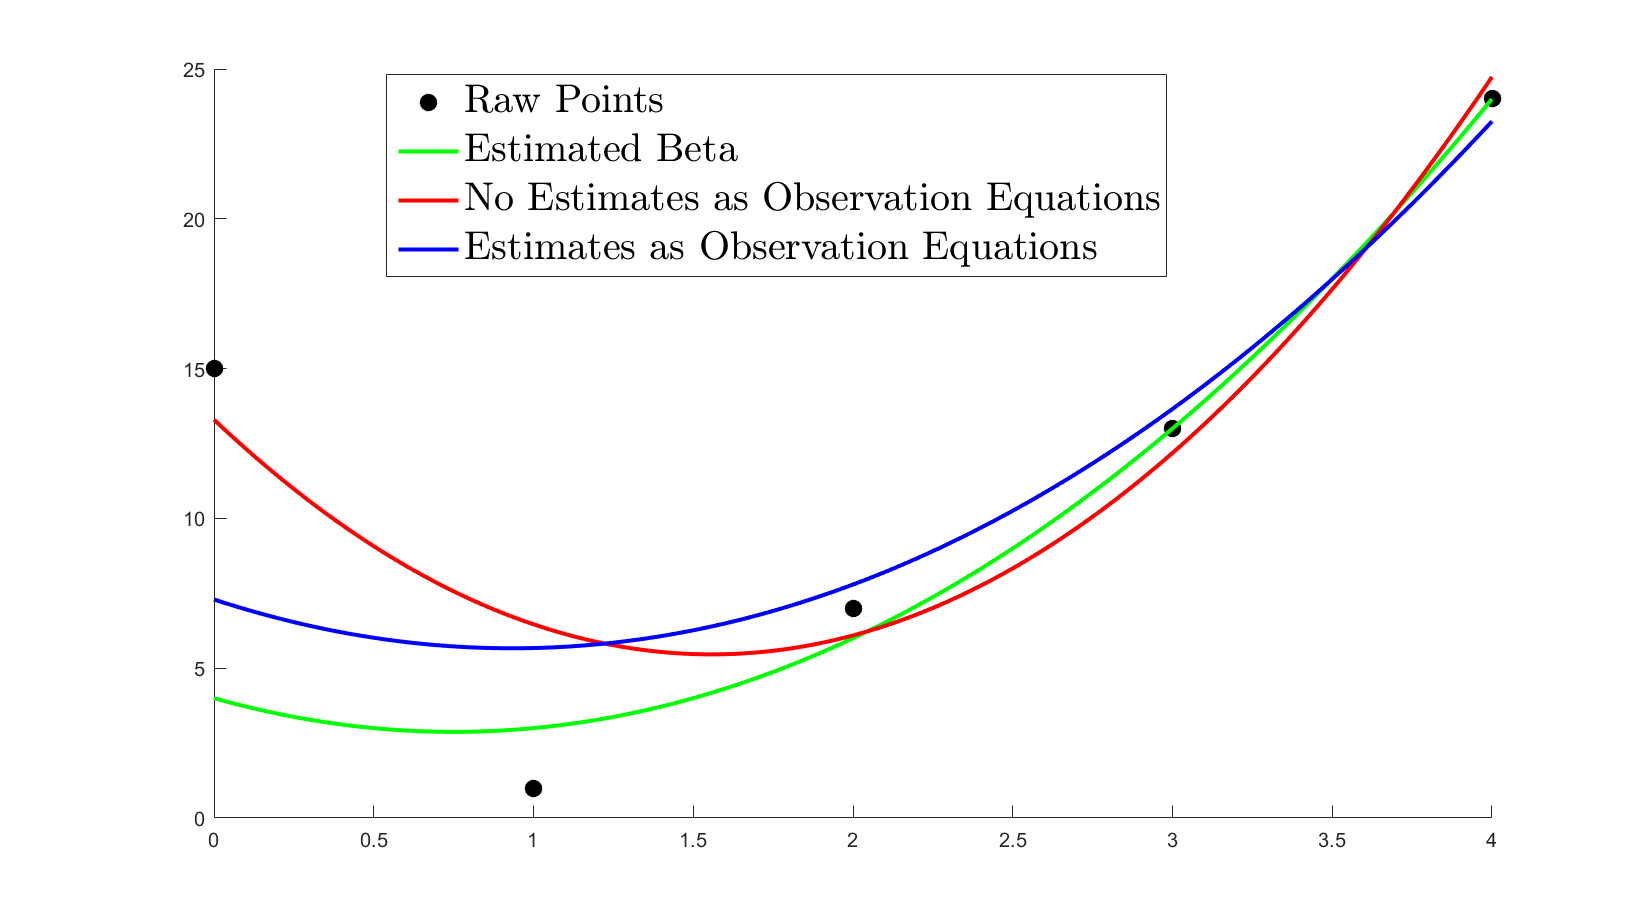
\includegraphics[width = \linewidth]{betacov}
	\end{figure}
	
	\clearpage
	\subsubsection*{Modify the DerivStep for Partial Derivatives}
	This example demonstrates how you can modify the step used for computing numerical partial derivatives.  While this option is available, it should only be used in very rare, specific cases.
	
	\lstinputlisting[
	label      = {alg:lsr2},
	style      = Matlab-editor,
	basicstyle = \mlttfamily,
	firstline  = 321,
	lastline   = 342,
	firstnumber= 321
	]{../exampleLsr.m}
	
	\clearpage
	\subsection*{Example of poor observation equations}
	This example demonstrates a poor observation equation for linear least squares.  Notice how using the linear least squares equations to solve the least squares solution, y is nowhere to be found in the solution.  In the case of linear least squares, y must be input as a response variable rather than a reactant if it is a constant and not multiplied by any beta coefficients.  When it is not multiplied by a beta coefficient, the Jacobian will not contain y, and y will not be factored into the equation.
	
	With Observation Equation:
	\begin{align*}
	0 = v &= mx + b - y \\
	0 = y &= \beta_1x_1 + \beta_2 - x_2 \\
	\end{align*}
	The Jacobian is:
	\[
	J_{yb} = 
	\begin{bmatrix}
	\dfrac{\partial y}{\partial \beta_1} & \dfrac{\partial y}{\partial \beta_2}
	\end{bmatrix}
	= 
	\begin{bmatrix}
	x_1 & 1
	\end{bmatrix}
	\]
	The Hessian is all 0s, which implies linear least squares.
	\[
	H = 
	\begin{bmatrix}[3]
	\dfrac{\partial^2 y}{\partial \beta_1^2} & \dfrac{\partial^2 y}{\partial \beta_1 \partial \beta_2} \\
	\dfrac{\partial^2 y}{\partial \beta_2 \partial \beta_1} & \dfrac{\partial^2 y}{\partial \beta_2^2} \\
	\end{bmatrix}
	= 
	\begin{bmatrix}
	0 & 0 \\
	0 & 0 \\
	\end{bmatrix}
	\]
	Recall for linear least squares:
	\begin{align*}
	A &= J_{y\beta} = \text{Partial Derivative of F with respect to }\beta \\
	WA\hat{\beta} &= Wy + WV\\
	\hat{\beta} &= (A^TWA)^{-1}A^TWy + WV\\
	\end{align*}
	Notice that $x_2$, does not factor into the equation at all! Refer to the nonlinear least squares equations and notice that the $K$ matrix will contain $x_2$ and therefore it will influence the solution.  
	
	\lstinputlisting[
	label      = {alg:lsr2},
	style      = Matlab-editor,
	basicstyle = \mlttfamily,
	firstline  = 344,
	lastline   = 363,
	firstnumber= 344
	]{../exampleLsr.m}
	
\end{document}